\chapter{Endpoint security}

\section{Endpoint security solutions}

Protecting endpoints in a borderless network can be accomplished using the following modern security solutions: Advanced Malware Protection (AMP), Email Security Appliance (ESA), Web Security Appliances (WSA), and Network Admission Control (NAC).

AMP defeats malware across the extended network before, during, and after an attack. AMP for Endpoints integrates with AMP for Networks to deliver comprehensive protection across extended networks and endpoints. \\

ESA fights spam, viruses, and blended threats. The Cisco ESA is constantly updated by real-time feeds from the Cisco Talos. Some of the main features and benefits of ESA: Global threat intelligence, Spam blocking, integrated with AMP, and Outbound message control.\\

WSA controls over how users access the Internet. It performs blacklisting, URL-filtering, malware scanning, Web application filtering, and TLS/SSL encryption and decryption. These are some of the main features and benefits of WSA: AMP, Data Loss Prevention (DLP), Talos security intelligence, and Web usage control.\\

Cloud Web Security (CWS) is a cloud-based security service that uses web proxies in Cisco’s cloud environment to scan traffic. Cisco devices can connect to CWS using a proxy autoconfiguration (PAC) file or through connectors integrated into four Cisco products: ISR G2 routers, ASA, WSA, and AnyConnect Secure Mobility Client.\\

NAC allows only authorized and compliant systems to access the network by providing authentication, authorization, and posture assessment. NACs are evolving to become more sophisticated endpoint visibility, access, and security (EVAS) controls.\\

There are two categories of Cisco NAC products: NAC framework and NAC appliance. The NAC framework uses the existing network infrastructure and third-party software to enforce security policy. The NAC Appliance incorporates NAC functions into an appliance.\\

NAC has three components: Manager, Server, and Agent. NAC Manager defines role-based user access and endpoint security policies. NAC Server (NAS) assesses and enforces security policy compliance. NAC Agent (NAA), which runs on an endpoint device, performs deep inspection of the device's security profile.\\

These are two additional TrustSec Policy enforcement tools for NAC: guest server and profiler. Guest server enforces guest network policy to either NAC appliance or Wireless LAN controller. It also provides the ability to create guest accounts. \\

On the other hand, NAC profiler enables the dynamic discovery, identification, and monitoring of all network-attached endpoints. It has two components: Collector and Server. Profiler server aggregates information from Collector and stores it in a database, then provisions the appropriate access decisions.

\begin{itemize}
\item Advanced Malware Protection (AMP) d
\item Email Security Appliance (ESA) = SPAM filtering
\item Web Security Appliances (WSA) = Blacklisting and URL filtering. WSA is a secure web gateway which combines AMP, application visibility and control, acceptable use policy controls, reporting, and secure mobility functions. 
\item Network Admission Control (NAC) = Data loss prevention. 
\item Cisco Cloud Web Security (CWS) is a cloud-based security service that uses web proxies in Cisco’s cloud environment to scan traffic for malware and policy enforcement. Cisco customers can connect to the Cisco CWS service through connectors integrated into four Cisco products: ASA, WSA, ISR G2 routers, and AnyConnect Secure Mobility Client.
\end{itemize}


\section{CAM table attack}

\textbf{CAM table overflow} attacks (also called MAC address overflow attacks) take place by bombarding the switch with fake source MAC addresses until the switch MAC address table is full. When this occurs, the switch treats the frame as an unknown unicast and begins to flood all incoming traffic to all ports. We prevent CAM table overflow using \textbf{port security} on access port.\\

The type of secure address can be Static, or Dynamic, or Sticky. Static secure MAC addresses are manually configured by the administrator and they are stored in both CAM table and running configuration. On the other hand, switches learn Dynamic addresses automatically but only keeps them in CAM table. Because CAM table locates in RAM, Dynamic addresses are removed when the switch restarts. \\

Sticky is the combination of static and dynamic types. Like static addresses, sticky addresses are stored in the address table and running configuration. Sticky learning is dynamic just like Dynamic type. Additionally, the switch converts all learned MAC addresses into sticky addresses. If sticky learning is disabled, the sticky secure MAC addresses remain part of the address table but are removed from the running configuration.

\begin{sexylisting}{Enable port security}
int g0/0
	sw mode access
	sw port-security
	sw port-security mac-address sticky 
	end	
show port-security
show port-security interface g0/0	
\end{sexylisting}




A security \textbf{violation} describes a situation when an unknown MAC address attempts to access an interface with port security configured. Whenever a violation occurs, the switch drops all frames associated with malicious MAC addresses. There are three violation modes: Protect, Restrict, and Shutdown. Only Shutdown mode is capable of putting port into error-disabled state. A detection of violation forces both Shutdown and Restrict mode send syslog message and increase violation counter. However, this is not the case for Protect mode.\\

You can bring a port in error-disabled state back to normal by entering \code{shutdown} followed by \code{no shutdown} command. 

\begin{sexylisting}{Additional port security}
int g0/0
	sw port-security max 2
	sw port-security violation mode shutdown
	sw port-security aging time 10
	sw port-security aging type inactivity
	exit
mac address-table notification	
\end{sexylisting}

To set the maximum number of MAC addresses allowed on a port use the \code{sw port-security max <value>}.\\

We use Port aging to remove secure MAC addresses on a secure port without manually deleting the existing secure MAC addresses. Two types of aging are supported per port: Absolute and Inactivity. Absolute aging deletes an address after the specified time, while Inactivity aging removes ports that is sleeping more than a specified of time.\\

The \textbf{MAC address notification} feature sends SNMP trap whenever a new MAC address is added to, or an old address is deleted from the CAM tables. This feature is only available for dynamic and secure MAC addresses.

\section{VLAN attacks}

\subsection{VLAN hopping and double-tagging}

A \textbf{VLAN hopping attack} enables traffic from one VLAN to be seen by another VLAN without the aid of a router. A VLAN hopping attack can be launched in one of two ways: Spoofing DTP messages or Introducing a rogue switch. Another type of VLAN attack is double-tagging. This attack method adds a hidden 802.1Q tag inside the frame which allows the frame to go to another VLAN. This attack works even if trunk ports are disabled.\\

The best way to prevent basic these attacks:

\begin{itemize}
\item Manually enable trunking and access ports
\item Disable DTP on trunking ports using the \code{sw non-negotiate}, on non-trunking port using \code{sw mode access}.
\item Set the native VLAN to be something other than VLAN 1
\item Be sure that native VLAN is only used for trunk lines.
\item Disable unused ports and put them in an unused VLAN.
\item Implement Private VLAN
\end{itemize}

\subsection{Priavte VLAN}

Private VLANs (PVLAN) provide Layer 2 isolation between hosts within the same VLAN. There are three types of PVLAN ports (figure \ref{PVLAN}): promiscuous, isolated, and community. A promiscuous port (often connected to the router) can talk to everyone. Community ports can talk to ports in the same community and promiscuous ports. An isolated port can only talk to promiscuous ports.


\begin{figure}[hbtp]
\caption{PVLANs -- promiscuous ports, isolated ports, community ports}\label{PVLAN}
\centering
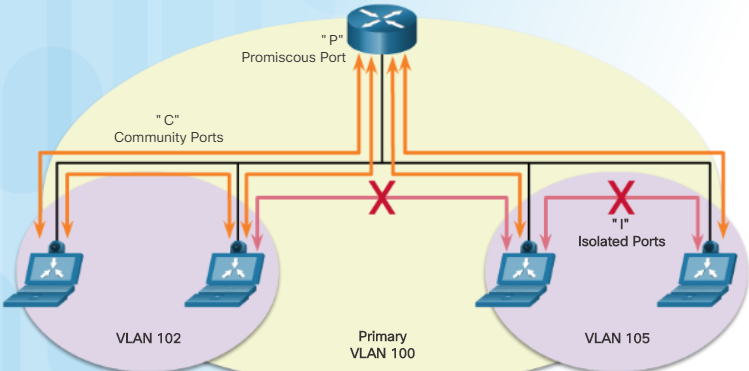
\includegraphics[scale=0.5]{pictures/PVLAN.PNG}
\end{figure}

%Full PVLAN support is available on 3560 Multiplayer switches or higher. The 2960 Switches only support a part of PVLAN (PVLAN Edge). \\

In creating full PVLAN, you need to create three special VLANs: primary VLAN (goes with the promiscuous ports), isolated VLAN, and community VLAN (can be different communities based on the VLAN number). Look at the figure \ref{PVLANconfig} for sample configuration. In order for PVLAN to work, you need to set VTP mode to transparent. 

\begin{figure}[hbtp]
\caption{Configuration of Private VLANS on a 3560 Multilayer switch}\label{PVLANconfig}
\centering
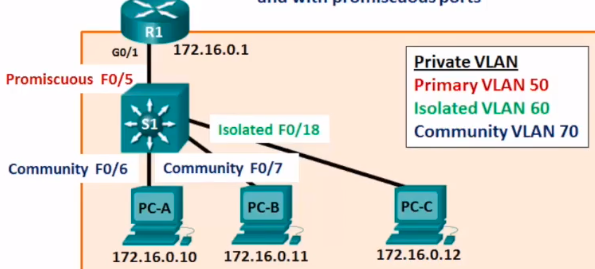
\includegraphics[scale=0.5]{pictures/PVLANconfig.PNG}
\end{figure}

\begin{sexylisting}{PVLAN}
vtp mode transparent

vlan 60
private-vlan isolated
vlan 70
private-vlan community
vlan 50
private-vlan primary
private-vlan association 60,70
exit

int f0/5
sw mode private-vlan promiscuous
sw private-vlan mapping 50 60,70
int f0/6
sw mode private-vlan host
sw private-vlan host-association 50 70
int f0/7
sw mode private-vlan host
sw private-vlan host-association 50 70
int f0/18
sw mode private-vlan host
sw private-vlan host-association 50 60
exit
\end{sexylisting}

If you only have a 2960 series switch and you do not have a multilayer switch, you can use the \code{sw protected} interface configuration command to achieve a similar result. Ports configured with this command is called Protected ports. Hosts connected to Protected ports will not be able to communicate with each other, but can only talk with un-Protected ports. 

\section{DHCP attacks}

\textbf{DHCP starvation} attack requires an attack tool, such as Gobbler, look at the entire pool of available IP addresses in DHCP and tries to lease them all (DoS attack). It is easy to mitigate DHCP starvation attacks using port security. \\

A \textbf{DHCP spoofing} attack occurs when a rogue DHCP server is connected to the network and provides false IP configuration parameters to legitimate clients. DHCP spoofing attacks can be mitigated using DHCP snooping on trusted ports. The general rule is that ports connected to hosts are untrusted, the other is trusted. Port connected to DHCP server must be trusted, otherwise DHCP service will not work.

\begin{figure}[hbtp]
\caption{Trusted and untrusted DHCP spoofing ports}\label{DHCPspoofing}
\centering
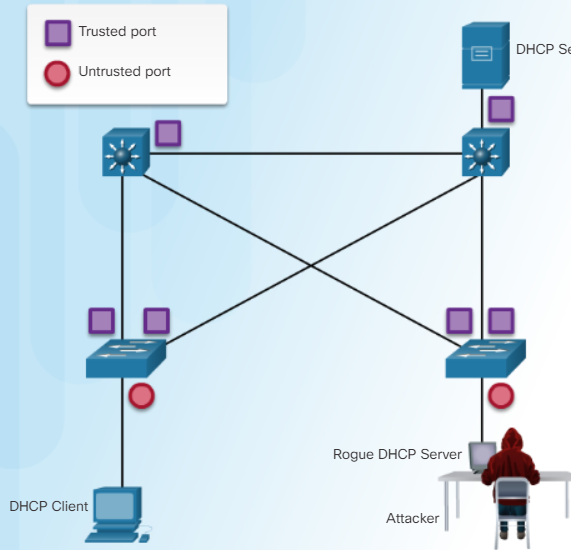
\includegraphics[scale=0.5]{pictures/DHCPspoofing.PNG}
\end{figure}

\begin{sexylisting}{DHCP snooping}
ip dchp snooping
 
int f0/1
ip dchp snooping trust
int range f0/5-24
ip dchp snooping rate 6
exit

ip dchp snooping vlan 5,10,20
\end{sexylisting}


\section{Dynamic ARP Inspection (DAI)}

An attacker can send a gratuitous ARP message containing a spoofed MAC address to a switch (ARP spoofing). \textbf{Dynamic ARP Inspection (DAI)} will be configured to mitigate against ARP spoofing and ARP poisoning attacks.

\begin{sexylisting}{Dynamic ARP Inspection (DAI) configuration}
ip dhcp snooping
ip dhcp snooping vlan 10
ip arp inspection vlan 10

int f0/24
ip dhcp snooping trust
ip arp inspection trust
exit

ip arp inspection validate src-mac
ip arp inspection validate dest-mac
ip arp inspection validate ip
ip arp inspection validate src-mac dest-mac ip
\end{sexylisting}

DHCP snooping is enabled because DAI requires the DHCP snooping table to operate. Next, DHCP snooping and ARP inspection are enabled for the PCs on VLAN10. The uplink port to the router is trusted, and therefore, is configured as trusted for DHCP snooping and ARP inspection.\\

The \code{ip arp inspection validate} global configuration command is used to configure DAI to drop ARP packets when the \code{ip}, or \code{src-mac} (source MAC address), or \code{dest-mac} (destination MAC address) are invalid. Notice that entering multiple \code{ip arp inspection validate} commands overwrite the previous command. To include more than one validation method, enter them on the same command line as displayed in the output.

\section{IP Source Guard (IPSG)}

To protect against MAC and IP address spoofing, configure the IP Source Guard (IPSG) security feature. IPSG operates just like DAI, but it looks at every packet, not just the ARP packets. Like DAI, IPSG also requires that DHCP snooping be enabled.\\

Specifically, IPSG is deployed on untrusted Layer 2 access and trunk ports using the \code{ip verify source} interface configuration command. IPSG dynamically maintains per-port VLAN ACLs (PVACL) based on IP-to-MAC-to-switch-port bindings. For each untrusted port, there are two possible levels of IP traffic security filtering:

\begin{itemize}
\item IP addresses -- only IP traffic with a source IP address that matches the IP source binding entry is permitted. 
\item IP and MAC address -- Only IP traffic with source IP and MAC addresses that match the IP source binding entry are permitted.
\end{itemize}

\section{Mitigating STP Attacks}

\subsection{PortFast}

The spanning-tree PortFast feature causes an interface configured as a Layer 2 access port to transition from the blocking to the forwarding state immediately, bypassing the listening and learning states. PortFast can be used on Layer 2 access ports that connect to a single workstation or server. Because the purpose of PortFast is to minimize the time that access ports must wait for STP to converge, it should be used only on access ports. \\

PortFast can be configured globally on all non-trunking ports using the \code{spanning-tree portfast default} global configuration command. Alternatively, PortFast can be enabled on an interface using the \code{spanning-tree portfast} interface configuration command.

\subsection{BPDU Guard}

Even though PortFast is enabled, the interface will listen for BPDUs. The receipt of unexpected BPDUs might be accidental, or part of an unauthorized attempt to add a switch to the network. BPDU Guard protects the integrity of ports that are PortFast-enabled. If any BPDU is received on a BPDU Guard enabled port, that port is put into error-disabled state. \\

Use the \code{spanning-tree portfast bpduguard} default global configuration command to globally enable BPDU guard on all PortFast-enabled ports. If PortFast is not configured, then BPDU Guard is not activated. Alternatively, BPDU Guard can be enabled per interface using the \code{spanning-tree bpduguard enable} interface configuration command.

\note Always enable BPDU Guard on all PortFast-enabled ports.

\subsection{Root Guard}

On a network, there are some switches that should never, under any circumstances, become the STP root bridge. Root Guard provides a way to enforce the placement of root bridges on the network by limiting which switch can become the root bridge. \\

Root guard is deployed on ports that \emph{toward} the unsecure switches (switches that should not be the root bridge). Look at figure \ref{RootLoopGuard}, we don't want S1 to be root bridge, so that F0/1 on both S2 and S3, which are towards S1, should be configured with Root Guard.\\

If a root-guard-enabled port receives BPDUs that are superior to those that the current root bridge is sending, that port is moved to a \emph{root-inconsistent state}. Recovery occurs as soon as the offending device ceases to send superior BPDUs.\\



\begin{figure}[hbtp]
\caption{Root and Loop Guard reference topology}\label{RootLoopGuard}
\centering
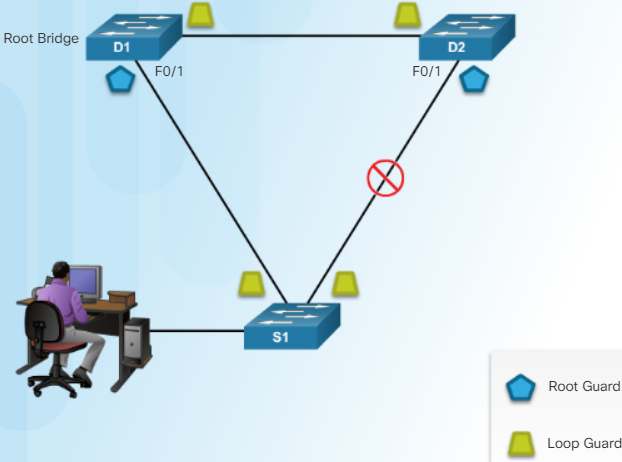
\includegraphics[scale=0.5]{pictures/RootLoopGuard.PNG}
\end{figure}


Use the \code{spanning-tree guard root} interface configuration command to configure root guard on an interface. To view Root Guard ports that have received superior BPDUs and are in a root-inconsistent state, use the \code{show spanning-tree inconsistent ports} command.\\

Root guard in conjunction with PortFast, and BPDU guard is used to prevent an STP manipulation attack.

\subsection{Loop Guard}

Traffic on bidirectional links flows in both directions. If for some reason one direction traffic flow fails, this creates a unidirectional link which can result in a Layer 2 loop. If BPDUs are not received on a non-designated Loop Guard-enabled port, the port transitions to a loop-inconsistent blocking state, instead of the listening / learning / forwarding state. \\

Loop Guard is enabled on all \emph{non-Root guard} ports (figure \ref{RootLoopGuard}) using the \code{spanning-tree guard loop} interface configuration command.